\section{Theorie}
\label{sec:Theorie}
\subsection{Abbildungsgesetz und Linsengleichung}
Trifft Licht auf eine Linse, so wird der Lichtstrahl nach dem Brechungsgesetz bei Eintritt und Austritt aus der Linse gebrochen.
Grund dafür, ist das Material der Linse, welches meistens optisch dichter als das Umgebungsmedium (Luft) ist.
\begin{figure}
\centering
\begin{subfigure}{0.48\textwidth}
    \centering
    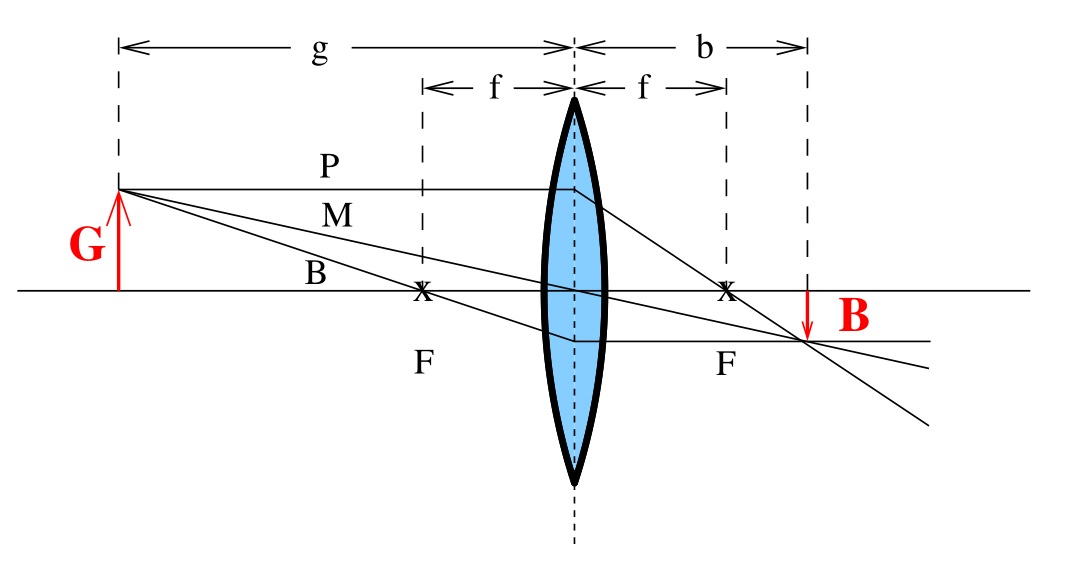
\includegraphics[width=0.9\linewidth]{content/data/sammellinse_duenn.jpg}
    \caption{Dünne Sammellinse}
    \label{fig:sammellinse_duenn}
\end{subfigure}
\begin{subfigure}{0.48\textwidth}
    \centering
    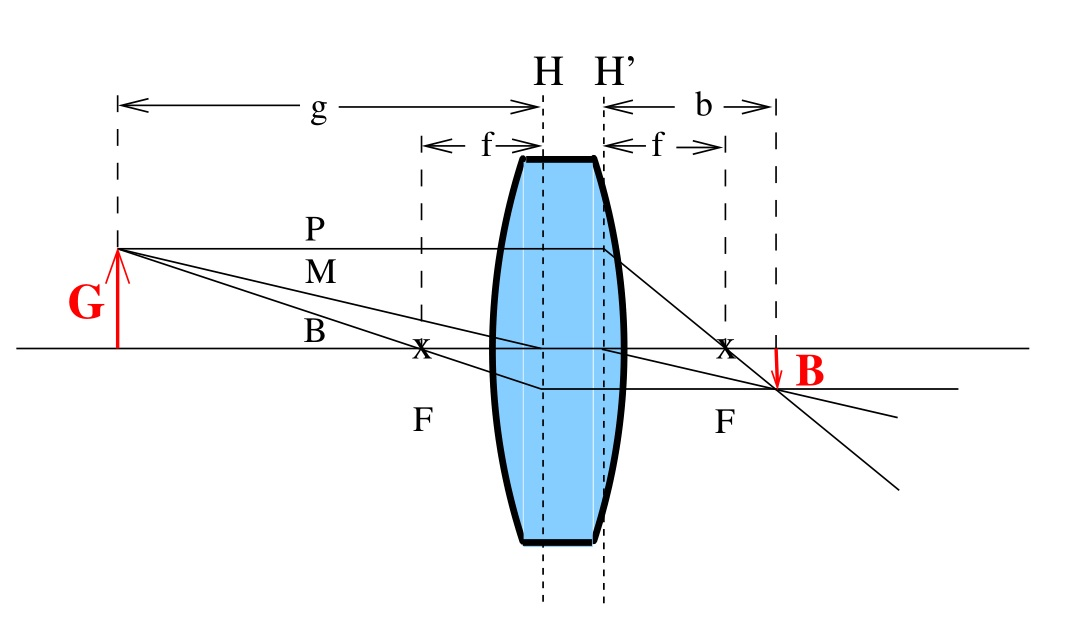
\includegraphics[width=0.9\linewidth]{content/data/sammellinse_dick.jpg}
    \caption{Dicke Sammellinse}
    \label{fig:sammellinse_dick}
\end{subfigure}
\caption{Eine schematische Darstellung einer dünnen und dicken Sammellinse. \cite[1]{anleitung}}
\label{fig:sammellinse}
\end{figure}

\begin{wrapfigure}{r}{0.5\linewidth}
    \centering
    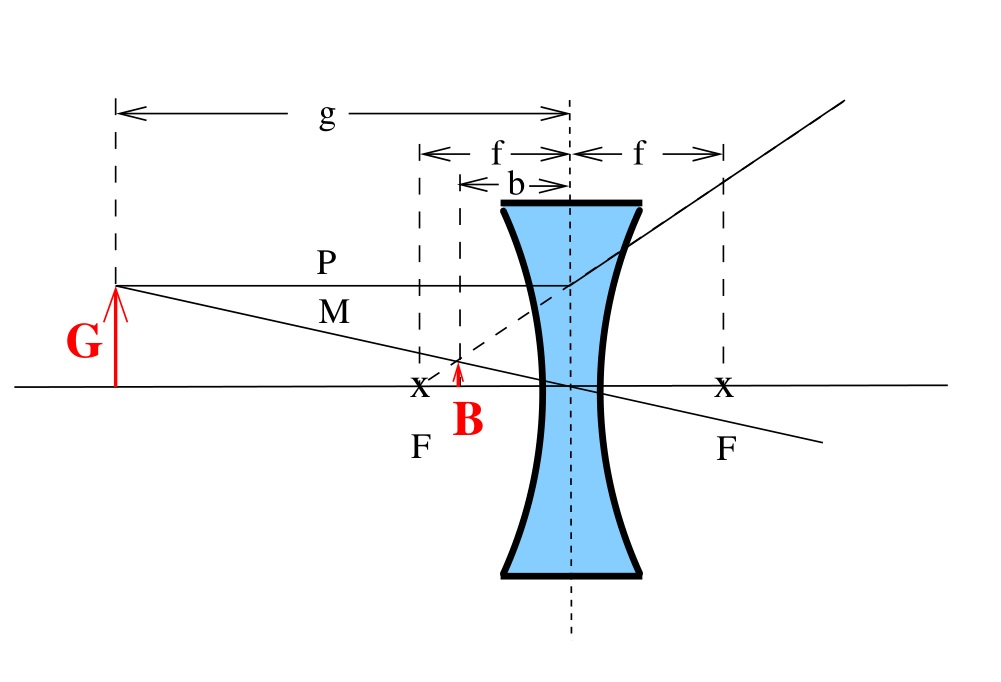
\includegraphics[width=0.9\linewidth]{content/data/zerstreuungslinse.jpg}
    \caption{Eine schematische Darstellung einer Zerstreuungslinse. \cite[1]{anleitung}}
    \label{fig:zerstreuungslinse}
\end{wrapfigure}
Linsen können in zwei Kategorien unterteilt werden.
Zum einen gibt es die Sammellinsen, welche in Abb. \ref{fig:sammellinse} dargestellt sind.
Sammellinsen bündeln parallele Lichtstrahlen in einem Punkt, dem Brennpunkt.
Sie haben eine positive Brennweite $f$ und Bildweite $b$.
Es entsteht ein reeles Bild, das auf einem Schirm abgebildet werden kann.
Bei einer dünnen Sammellinse (Abb. \ref{fig:sammellinse_duenn}) kann angenommen werden, dass das Licht in der Mittelebene gebrochen wird.
Anders bei dicken Linsen.
Hier werden zwei sogenannte Hauptebenen eingeführt, an denen die Lichtstrahlen gebrochen werden.
\\
Die Zerstreuungslinse (siehe Abb. \ref{fig:zerstreuungslinse}) hat im Gegensatz zur Sammellinse eine negative Brennweite $f$ und Bildweite $b$.
Es entsteht ein virtuelles Bild, welches nicht auf einem Schirm sichtbar ist.
\\
Zur Bildkonstruktion werden folgende Strahlen definiert:
\begin{description}
    \item[Parallelstrahl P] verläuft parallel zur optischen Achse vom Gegenstand zur Mittel- bzw. Hauptebene, wird gebrochen und verläuft weiter als Brennpunktstrahl
    \item[Mittelpunktstrahl M] verläuft vom Gegenstand durch die Mitte der Linse und wird nicht gebrochen
    \item[Brennpunktstrahl B] geht durch den Brennpunkt der Linse, wird dann an der Mittel- bzw. Hauptebene gebrochen und verläuft weiter parallel zur optischen Achse
\end{description}
Das Abbildungsgesetz
\begin{equation}
    V = \frac{B}{G} = \frac{b}{g}
    \label{eqn:abbildungsgesetz}
\end{equation}
beschreibt den Abbildungsmaßstab $V$.
Die Bildgröße $B$ und Gegenstandgröße $G$ stehen also im gleichen Verhältnis, ie die Bildweite $b$ und Gegenstandweite $g$.
Für dünne Linsen folgt aus dem Abbildungsgesetz und der Bildkonstruktion die Linsengleichung
\begin{equation}
    \frac{1}{f} = \frac{1}{b} + \frac{1}{g} \, .
    \label{eqn:linsengleichung}
\end{equation}
Wie oben erwähnt, wird bei Dicken Sammellinsen die Mittelebene durch zwei gedachte Hauptebenen $H$ und $H'$ ersetzt.
Die Linsengleichung \ref{eqn:linsengleichung} behält ihre Gültigkeit, wenn die Brennweite, Gegenstandsweite und die Bildweite zur jeweiligen Hauptebene definiert wird.
\\
Allgemein gilt die Reduzierung der Brechung auf eine Mittelebene bzw. Hauptebene nur für achsennahe Strahlen.
Treffen achsenferne Strahlen auf die Linse, so werden diese stärker gebrochen und treten Abbildungsfehler auf.
Bei der spährischen Abberration liegt der Brennpunkt achsenferner Strahlen näher an der Linse als bei achsennahen Strahlen.
Das Bild wird nicht mehr scharf auf einem Schirm abgebildet.
Mithilfe bestimmter Blenden (z.B. Irisblende) können achsenferne Strahlen ausgeblendet und ein scharfes Bild erzeugt werden.
\\
Die chromatische Abberration entsteht, wenn Licht unterschiedlicher Wellenlängen auf die Linse triftt.
Das Licht wird unterschiedlich stark gebrochen.
Zum Beispiel liegt der Brennpunkt vom blauen Licht näher an der Linse als vom roten, da das blaue Licht stärker gebrochen wird.
\\
Die Brechkraft $D=\frac{1}{f}$ hat die Einheit Dioptrie $[\text{dpt}=\si{\frac{1}{\metre}}]$ und wird durch die reziproke Brennweite $f$ definiert.
Befinden sich mehrere dünne Linsen in einem Aufbau, so spricht man von einem Linsensystem und die Brechkraft ergibt sich aus den einzelnen Brechkräften der Linsen $D_i$
\begin{equation}
    D = \sum_i^N D_i \, .
    \label{eqn:linsensystem}
\end{equation}
\FloatBarrier
\newpage

\subsection{Methode von Bessel}
\begin{wrapfigure}{r}{0.5\linewidth}
    \centering
    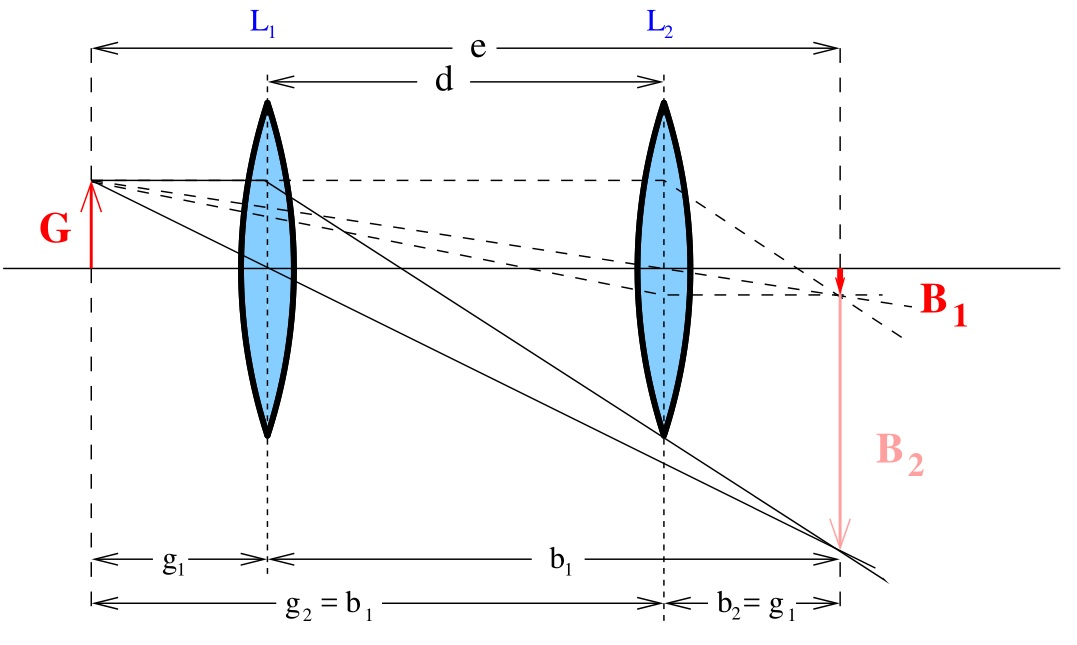
\includegraphics[width=0.9\linewidth]{content/data/bessel.jpg}
    \caption{Eine schematische Darstellung zweier Linsen zur Bestimmung der Brennweite nach der Methode von Bessel. \cite[4]{anleitung}}
    \label{fig:bessel}
\end{wrapfigure}
Der Abstand zwischen Gegenstand und Bild wird konstant gehalten.
Es gibt nun zwei Positionen der beiden Linsen, bei denen das Bild scharf ist.\\
Die Gegenstandweite und Bildweite werden dabei vertauscht (symmetrische Linseneinstellung):
\begin{align*}
    b_1 &= g_2 \\
    b_2 &= g_1 \\
\end{align*}
Gilt $g > b$ so ist das Bild verkleinert.
Wenn die Gegenstandsweite kleiner als die Bildweite ist $g < b$, wird das Bilder vergrößert.
Es werden die Größen $e = g_1 + b_1 = g_2 + b_2$ zwischen Gegenstand und Bild, sowie $d = g_1 - b_1 = g_2 - b_2$ dem Abstand zwischen der 1. und 2. Linse definiert (siehe Abb. \ref{fig:bessel}).
Die Brennweite der Linse wird nach
\begin{equation}
    f = \frac{e^2 - d^2}{4e}
    \label{eqn:bessel}
\end{equation}
bestimmt.
\FloatBarrier

\subsection{Methode von Abbe.}
Nach der Methode von Abbe. wird die Brennweite bzw. die Lage der Hauptebenen aus dem Abbildungsmaßstab $V$ bestimmt.
Die Hauptebenen $H$ und $H'$ der dicken Linse sind nicht bekannt, daher wird die Gegenstandsweite $g'$ und Bildweite $b'$ zu einem beliebigen Punkt $A$ gemessen.
Für das Linsensystem gelten die folgenden Gleichungen:
\begin{align}
    g' = g + h = f \cdot \left( 1+ \frac{1}{V} \right) + h \\
    b' = b + h' = f \cdot \left( 1 + V \right) + h'
    \label{eqn:abbe}
\end{align}
Dabei steht $V$ für den Abbildungsmaßstab und $g'$ und $b'$ für die gemessenen Abstände.
Aus den Größen kann die Brennweite $f$ und die Lage der Hauptebenen bestimmt werden.